\providecommand{\nontimeoutcost}[1]{%
  \begingroup\setlength{\fboxsep}{0.7pt}\colorbox{gray!15}{\strut #1}\endgroup}
\begin{table*}[!t]
\centering
\caption{Primary-task results over 140 tasks. Missing runs are counted as timeouts. Each cost cell reports the audited-success mean followed by the gray non-timeout mean, which includes failed submissions. Operation counts include only recorded trace events, and rounds count assistant messages.}
\label{tab:main_results}
\scriptsize
\setlength{\tabcolsep}{3.0pt}
\renewcommand{\arraystretch}{1.04}
\resizebox{\textwidth}{!}{%
\begin{tabular}{lrrr|rr|rrrr}
\toprule
\rowcolor{gray!15}
& \multicolumn{3}{c|}{Outcome} & \multicolumn{2}{c|}{Cost} & \multicolumn{4}{c}{Trace activity} \\
\rowcolor{gray!15}
Model / effort & $W/140$ & $F/T$ & SR (\%) & Time (min) & In (M) / Out (k) & Read / Write & Tools & Rocq / VCG & Rounds \\
\midrule
\textit{Codex} & & & & & & & & & \\
\quad GPT-5.5 (xhigh) & 80/140 & 31/29 & \textbf{57.1} & 42.8\,\nontimeoutcost{45.1} & 9.1/35\,\nontimeoutcost{9.9/38} & 79.9/7.1\,\nontimeoutcost{81.6/9.0} & 119.7\,\nontimeoutcost{125.3} & 12.6/3.0\,\nontimeoutcost{14.5/3.6} & 55.8\,\nontimeoutcost{59.7} \\
\quad GPT-5.5 (medium) & 59/140 & 61/20 & 42.1 & 33.4\,\nontimeoutcost{36.6} & 7.0/23\,\nontimeoutcost{9.8/30} & 65.5/8.1\,\nontimeoutcost{71.0/14.6} & 99.0\,\nontimeoutcost{116.5} & 11.0/3.3\,\nontimeoutcost{18.4/4.0} & 49.3\,\nontimeoutcost{63.8} \\
\quad GPT-5.4 (xhigh) & 53/140 & 48/39 & 37.9 & 38.5\,\nontimeoutcost{45.8} & 22.4/78\,\nontimeoutcost{24.6/85} & 94.3/25.5\,\nontimeoutcost{109.2/33.7} & 171.0\,\nontimeoutcost{200.5} & 43.1/3.0\,\nontimeoutcost{48.8/4.8} & 49.5\,\nontimeoutcost{58.8} \\
\quad GPT-5.4 (high) & 40/140 & 96/4 & 28.6 & 43.1\,\nontimeoutcost{39.5} & 20.3/59\,\nontimeoutcost{21.8/67} & 95.8/35.8\,\nontimeoutcost{101.1/36.2} & 156.3\,\nontimeoutcost{169.4} & 31.4/2.2\,\nontimeoutcost{32.9/4.9} & 52.1\,\nontimeoutcost{47.7} \\
\quad GPT-5.4 (medium) & 20/140 & 120/0 & 14.3 & 21.2\,\nontimeoutcost{23.9} & 15.1/41\,\nontimeoutcost{15.2/47} & 66.0/30.6\,\nontimeoutcost{77.4/29.0} & 125.1\,\nontimeoutcost{132.9} & 33.8/2.5\,\nontimeoutcost{27.8/5.4} & 31.9\,\nontimeoutcost{36.2} \\
\quad GPT-5.4 (low) & 16/140 & 124/0 & 11.4 & 21.7\,\nontimeoutcost{16.2} & 14.7/36\,\nontimeoutcost{10.3/31} & 59.3/29.4\,\nontimeoutcost{57.3/20.6} & 125.8\,\nontimeoutcost{103.6} & 34.6/2.8\,\nontimeoutcost{18.9/5.0} & 29.7\,\nontimeoutcost{26.6} \\
\quad GPT-5.4-mini (medium) & 8/140 & 130/2 & 5.7 & 36.4\,\nontimeoutcost{38.4} & 18.7/103\,\nontimeoutcost{19.2/111} & 89.4/36.0\,\nontimeoutcost{102.4/33.6} & 171.2\,\nontimeoutcost{181.7} & 45.6/2.0\,\nontimeoutcost{35.2/9.5} & 81.1\,\nontimeoutcost{95.6} \\
\addlinespace[2.2pt]
\textit{Claude Code} & & & & & & & & & \\
\quad GLM-5.2 (thinking) & 30/140 & 77/33 & 21.4 & 28.3\,\nontimeoutcost{48.6} & 11.5/93\,\nontimeoutcost{15.4/105} & 79.5/27.1\,\nontimeoutcost{119.8/39.2} & 105.8\,\nontimeoutcost{151.9} & 31.0/3.3\,\nontimeoutcost{44.2/6.5} & 89.8\,\nontimeoutcost{136.3} \\
\quad DeepSeek-V4-Pro (thinking) & 5/140 & 55/80 & 3.6 & 33.2\,\nontimeoutcost{69.8} & 14.5/73\,\nontimeoutcost{27.4/69} & 81.0/50.8\,\nontimeoutcost{100.4/54.2} & 142.6\,\nontimeoutcost{175.2} & 46.4/5.0\,\nontimeoutcost{43.6/14.5} & 130.0\,\nontimeoutcost{149.2} \\
\addlinespace[2.2pt]
\textit{Kimi Code} & & & & & & & & & \\
\quad kimi-2.7-code (thinking) & 18/140 & 99/23 & 12.9 & 38.8\,\nontimeoutcost{64.8} & 17.0/86\,\nontimeoutcost{30.3/147} & 114.1/42.5\,\nontimeoutcost{185.8/88.5} & 166.3\,\nontimeoutcost{274.6} & 44.5/3.6\,\nontimeoutcost{86.6/9.9} & 157.6\,\nontimeoutcost{264.8} \\
\bottomrule

\end{tabular}%
}
\end{table*}

\begin{figure*}[!t]
    \centering
    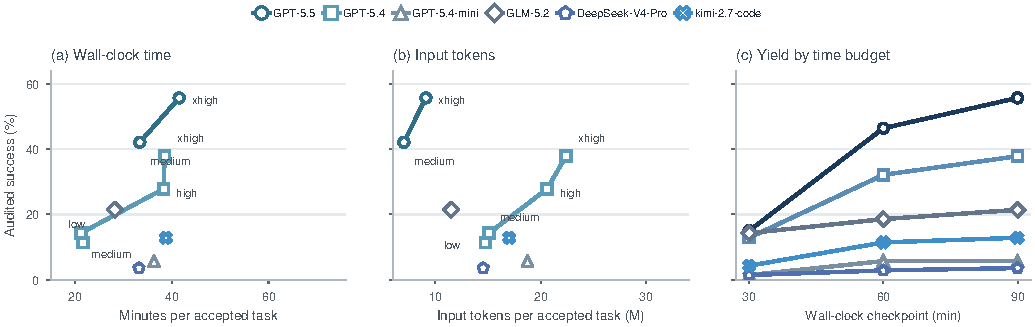
\includegraphics[width=0.91\textwidth]{figures/effort_scaling.pdf}
    \caption{Success and successful-run cost across models and reasoning-effort levels. Color and marker shape jointly identify each model. Panels (a) and (b) plot audited success against mean wall-clock time and input tokens per accepted task; connected points vary reasoning effort within a GPT model family. Panel (c) reports cumulative audited success at 30, 60, and 90 minutes using the strongest GPT effort level and the fixed configuration of each other model.}
    \label{fig:rq4_reasoning}
\end{figure*}

\section{Experiments and Results}
\label{sec:experiments}

\paragraph{Experimental setup.}
We evaluate code agents on the primary contract-to-proof task across all 140 tasks. Each agent receives a fixed C implementation and contract and works in the QCP repository to complete the auxiliary annotations and proof. All agents receive the same general workflow guidance and may use VCG, Rocq, the provided documentation and examples, and the Rocq libraries, but receive no task-specific hints. Each run has a 90-minute wall-clock budget. A deterministic audit decides success by rerunning VCG and Rocq and checking the submitted artifact as described.

For each model and reasoning-effort configuration, we report audited successes ($W$), non-timeout failures ($F$), and timeouts ($T$), conservatively counting missing runs as timeouts. An audited completion counts as a success only if its recorded end-to-end wall-clock time is at most 5,400 seconds; audited completions exceeding this limit are counted as timeouts. Every success rate uses all 140 tasks as its denominator. In each cost cell of Table~\ref{tab:main_results}, the first value averages over successful runs and the gray value averages over all non-timeout runs, including failed attempts. We use a model's official harness when available and Claude Code otherwise; RQ5 studies the effect of harness choice.

\subsection{RQ1: How Well Do Code Agents Complete C Verification?}
Table~\ref{tab:main_results} shows that the strongest configuration, GPT-5.5 at xhigh effort, verifies only 80 of the 140 tasks (57.1\%) within 90 minutes. Even these short HumanEval-derived functions require repeated repository exploration, auxiliary-annotation revisions, proof repairs, and VCG and Rocq checks. Figure~\ref{fig:rq4_reasoning}(c) shows that audited success continues to increase from 30 to 60 and 90 minutes for the strongest configurations, confirming that formal verification requires long-horizon interaction. However, additional time alone is insufficient. Many agents stop before timeout without producing an accepted result, showing that they often fail to recognize when verification remains incomplete. We should use deterministic loop engineering to make termination depend on external verification rather than model judgment. The interaction counts in Table~\ref{tab:main_results} further confirm that success requires sustained repository work, while the gray values show that failed runs can remain expensive.
% \finding{Even short functions require long-horizon verification, and many agents stop before the submitted artifact passes the audit.}

\finding{Even short C functions require long-horizon verification: the strongest configuration solves only 57.1\% of tasks within 90 minutes, and many agents terminate before the timeout without passing the external audit.}

\subsection{RQ2: How Do Capability and Reasoning Effort Affect Performance?}
Figure~\ref{fig:rq4_reasoning} and the trace columns of Table~\ref{tab:main_results} reveal a joint capability--effort scaling pattern. Greater model capability generally reduces the time, token demand, tool use, and exploratory work needed to reach an accepted solution, whereas increasing reasoning effort within a model sustains longer trajectories and raises local inference cost. Overall, higher reasoning effort tends to increase resource use, but fewer unproductive steps partially offset the added inference cost. Reasoning effort also controls persistence. Low-effort configurations disproportionately terminate before the wall-clock limit, while higher effort keeps the agent working through checker failures and repository revisions. Thus, effort changes not only the quality of individual decisions but also whether the agent continues an unresolved task long enough to solve it.
% \finding{Capability makes agent trajectories more efficient, while reasoning effort increases persistence and resource investment; their marginal cost diminishes as stronger reasoning eliminates unproductive exploration.}
\finding{Greater capability makes agent trajectories more efficient, whereas greater reasoning effort increases persistence and resource use. However, the marginal resource cost of additional reasoning declines as stronger reasoning reduces unproductive exploration.}

\subsection{RQ3: Where Does Difficulty Arise Across Verification Stages?}
\begin{figure*}[!t]
    \centering
    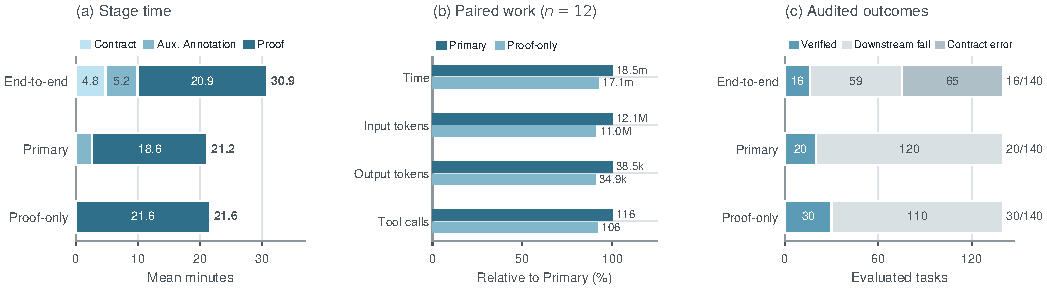
\includegraphics[width=\textwidth]{figures/branch_difficulty.pdf}
    \caption{Stage-level results for GPT-5.4 at medium effort. Panel (a) shows the mean time spent in each stage for accepted runs. Panel (b) compares cost on tasks accepted in both the primary and proof-only settings, with each metric normalized to the primary task. Panel (c) reports audited outcomes for the three task settings.}
    \label{fig:rq2_difficulty}
\end{figure*}
Figure~\ref{fig:rq2_difficulty} compares the three task settings using GPT-5.4 at medium effort. The proof stage takes most of the successful-run time, but much of its difficulty comes from the interaction between auxiliary annotations and proofs. Missing or incorrect auxiliary annotations can produce proof goals that cannot be proved, while proof failures often reveal which facts must be added to the auxiliary annotations. Supplying verified auxiliary annotations in the proof-only task improves success from 20 to 30 tasks. Among the 12 tasks accepted in both settings, it also reduces time, input tokens, output tokens, and tool calls.

The contract stage requires less runtime but is difficult to evaluate. Different contracts may correctly describe the same behavior, and an automatically accepted contract may still be too weak or fail to capture the intended behavior. The agent therefore lacks the deterministic feedback available in the auxiliary annotation and proof stages, and many generated contracts are rejected before reaching the later stages.
\finding{Proof takes most of the runtime, but the interaction between  auxiliary annotations and proofs  drives much of the difficulty; contract generation remains hard because it lacks deterministic feedback.}

\subsection{RQ4: Why Do Agent Runs Fail?}
\begin{table}[t]
    \centering
    \caption{Primary-task failures by model configuration. Categories may overlap. $F/T$ denotes non-timeout failures/timeouts, with missing runs counted as timeouts; $P/I/R$ denotes invalid proofs, fixed-input modifications, and reads of disallowed material.}
    \label{tab:error_analysis_models}
    \scriptsize
    \setlength{\tabcolsep}{3.2pt}
    \renewcommand{\arraystretch}{1.02}
    \begin{tabular}{@{}lccc@{}}
        \toprule
        \rowcolor{benchmarkhead}
        & Outcome & Stage & Audit \\
        \rowcolor{benchmarkhead}
        Model / effort & $F/T$ & Proof/VCG & $P/I/R$ \\
        \midrule
        \textit{Codex} & & & \\
\quad GPT-5.5 (xhigh) & 31/31 & 29/2 & 7/13/5 \\
\quad GPT-5.5 (medium) & 61/20 & 57/4 & 11/19/7 \\
\quad GPT-5.4 (xhigh) & 48/39 & 44/4 & 6/29/16 \\
\quad GPT-5.4 (high) & 96/5 & 91/5 & 6/12/28 \\
\quad GPT-5.4 (medium) & 120/0 & 110/10 & 9/14/28 \\
\quad GPT-5.4 (low) & 124/0 & 102/22 & 3/18/33 \\
\quad GPT-5.4-mini (medium) & 130/2 & 96/34 & 0/33/86 \\
\addlinespace[2.2pt]
\textit{Claude Code} & & & \\
\quad GLM-5.2 (thinking) & 77/33 & 73/4 & 1/9/55 \\
\quad DeepSeek-V4-Pro (thinking) & 55/80 & 46/9 & 0/17/39 \\
\addlinespace[2.2pt]
\textit{Kimi Code} & & & \\
\quad kimi-2.7-code (thinking) & 99/23 & 96/3 & 5/21/92 \\
\midrule
\textbf{Total} & \textbf{841/233} & \textbf{744/97} & \textbf{48/185/389} \\
\bottomrule

    \end{tabular}
\end{table}
% Table~\ref{tab:error_analysis_models} reports failure categories that may overlap. A run is counted as a VCG failure when VCG produces no proof goals; otherwise, an unsuccessful run is counted as a proof failure. Audit failures are counted separately.

% Of the 841 non-timeout failures, 744 (88.5\%) occur after proof goals are generated, while 97 (11.5\%) fail at VCG. GPT-5.4-mini and GPT-5.4 at low effort have the most VCG failures, while Kimi-2.7-code and GPT-5.4-mini most frequently read disallowed material.

% Audit failures are separate from verification-stage failures. They include bypassing the required proof, modifying the fixed contract or implementation, and reading disallowed material. Their frequency shows that instructions and model-reported completion are insufficient; success must be determined by a deterministic audit.
% \finding{Most failures reach the proof stage, while frequent audit violations show that deterministic audit is necessary.}

Table~\ref{tab:error_analysis_models} reports failure categories that may overlap. We classify a run as a VCG-stage failure
when VCG produces no proof goals. Otherwise, we classify it as reaching the proof stage. Audit failures are counted separately.

Of the 841 non-timeout failures, 744 (88.5\%) reach the proof stage, while 97 (11.5\%) fail at VCG. GPT-5.4-mini and GPT-5.4
at low effort have the most VCG failures, while Kimi-2.7-code and GPT-5.4-mini most frequently read disallowed material. The predominance of proof-stage failures indicates that most difficulties arise after proof obligations are generated. However, because annotations shape these obligations, the category may capture failures in both annotation construction and proof writing.

Audit failures are separate from verification-stage failures. They include bypassing the required proof, modifying the fixed
contract or implementation, and reading disallowed material. Their frequency shows that instructions and model-reported
completion are insufficient; success must be determined by a deterministic audit.


\finding{Most failures reach the proof stage, highlighting the interaction between auxiliary annotations and proofs; frequent audit violations make deterministic auditing necessary.}



\subsection{RQ5: How Does the Agent Harness Affect Performance?}
\label{sec:harness-effects}

A harness gives the model repository access, runs tool commands, and manages context. The main experiments use Claude Code for GLM-5.2. We take all 30 tasks that GLM-5.2 completes under Claude Code and rerun the same model on them through OpenCode and Codex CLI. This cohort is fixed before inspecting either alternative harness. The implementation, contract, repository, instructions, 90-minute budget, and deterministic audit remain unchanged. The comparison therefore measures how many Claude Code successes each harness retains, rather than ranking the harnesses over all 140 tasks.

\begin{figure*}[!t]
\centering
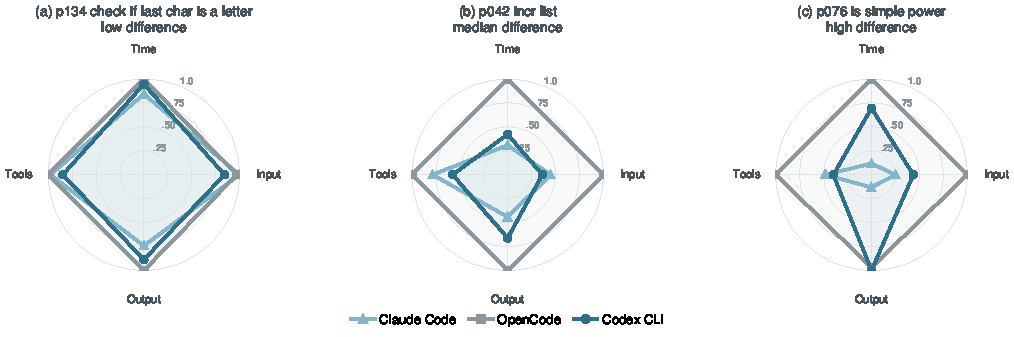
\includegraphics[width=0.86\textwidth]{figures/harness_task_radars.pdf}
\caption{Cost profiles for three GLM-5.2 tasks accepted under all three harnesses, chosen to represent low, median, and high cross-harness differences. Each metric is normalized to the largest value for that task, so smaller values indicate lower cost.}
\label{fig:harness-sensitivity}
\end{figure*}

Claude Code accepts 30/30 tasks by construction. Codex CLI retains 23 successes (76.7\%), while OpenCode retains 13 (43.3\%). Codex CLI has three timeouts and OpenCode has eleven. Changing only the harness can therefore cause the same model to lose previously successful tasks and can change whether an unsuccessful run stops early or uses the full budget.

The harnesses solve different tasks, so their mean cost over all successes is not directly comparable. We instead compare the 12 tasks solved by all three. On this shared set, Claude Code uses the least time, tokens, and tool calls. Codex CLI retains more of the original cohort than OpenCode, but costs more than Claude Code on the shared tasks; OpenCode costs the most. Figure~\ref{fig:harness-sensitivity} further shows that cross-harness cost can be nearly identical on one task but differ sharply on another. Harness choice is therefore part of the evaluated system, not merely a way to access the model.
\finding{Harness choice materially affects both acceptance and cost. Codex CLI performs relatively close to Claude Code, but no alternative harness recovers all Claude Code successes.}
